\cotefile{123}
\scanpage{2}
Complements on the Coxeter transformation of an \inserted{\handwritten{irreducible}} root system (Kostant).
\margin{\handwritten{The principal 3-dimensional subgroup ....\quad th. 9.2.}}
% The insertion above the title is enclosed in an oval, with a leader to after ``racines''.
\margin{\handwritten{\figure{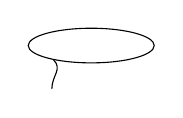
\begin{tikzpicture}[x=1cm,y=1cm]\draw (0,0) ellipse (0.8 and 0.22);\draw (-0.48,-0.18) .. controls (-0.36,-0.3) and (-0.5,-0.38) .. (-0.5,-0.55);\end{tikzpicture}}}}

a) Let $w\handwritten{\in}W$. Then every eigenvalue of $w$ \deleted{\unsure{di}}is a root of $1$ of order dividing one of the integers $m_i+1$ (where the $m_i$ are the characteristic exponents), hence of order $\handwritten{\leq}h$. For there to be one that is of order $h$, it is necessary and sufficient that $w$ be a Coxeter transformation, and\inserted{then} the nonzero elements of the corresponding eigenspace\handwritten{\tikz[baseline=.1ex,x=1em,y=1em]{\draw (0,0) circle (.13);\draw (.09,.1)--(.72,.9);}}\inserted{\handwritten{(which is of dimension $1$)}} are regular elements.
% A right marginal bracket holds the paragraph a).
\margin{\handwritten{\figure{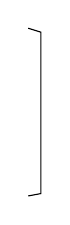
\begin{tikzpicture}[x=1cm,y=1cm]\draw (-0.16,0.05)--(0,0)--(0,-2.05)--(-0.16,-2.08);\end{tikzpicture}}}}

\uline{Corollary}\handwritten{1}: Let $\handwritten{\mu}$ be the subgroup of $W$ generated by a Coxeter element $c$, hence $\handwritten{\mu\simeq}\underline{Z}\handwritten{/}h\underline{Z}$. Then $\handwritten{\mu}$ is equal to the centralizer of $c$, hence of $\handwritten{\mu}$, and if $\handwritten{\nu}$ is the normalizer of $\handwritten{\mu}$, the homomorphism
% A left marginal rule holds the corollary through ``mod mu''.
\margin{\handwritten{\figure{\begin{tikzpicture}[x=1cm,y=1cm]\draw (0,0)--(0,-2.4);\end{tikzpicture}}}}
\[
\handwritten{\unsure{\psi|\nu}/\mu\longrightarrow}\operatorname{Aut}(\handwritten{\mu})\handwritten{\simeq}(\underline{Z}/h\underline{Z})^{\handwritten{*}}
\]
\margin{\handwritten{What extension of $(\unsure{Z|\mathbb{Z}}/hZ]^{*}$ by $Z/hZ$ does one obtain?}}
is a\deleted{j}n isomorphism; in other words, for every integer $n$ prime to $h$, there exists a $w\handwritten{\in}W$ such that $wcw^{-1}=c^h$, and $w$ is determined modulo $\handwritten{\mu}$.
\margin{\handwritten{\unsure{interchange|interchange} with corollary \unsure{3|?}}}

Let \deleted{\unsure{D|B}}in ef\inserted{\handwritten{f}}ect $D$ be \deleted{\unsure{a line}}\inserted{the subspace} of eigenvectors under $c$ corresponding to a primitive $h$-th root of $1$. Then $\dim D=1$ (Proposition 30), and $\handwritten{\mathfrak{z}}=\operatorname{Centr}(\handwritten{\mu})$ normalizes $D$, whence a homomorphism $\handwritten{\mathfrak{z}\to}\operatorname{Aut}(D)=\underline{C}^{\handwritten{*}}$, whose image is a finite subgroup of $\underline{C}^{\handwritten{*}}$, containing the image (isomorphic) of $\handwritten{\mu}$, hence cyclic of order a multiple of $h$. Thanks to Kostant, its order is equal to $h$, and we have thus found a retraction $\handwritten{\mathfrak{z}\to\mu}$, we must prove that its kernel is reduced to $1$. Now if $w$ is in this kernel, it \deleted{induces} centralizes $D$, and \unsure{since|since} $D$ is regular by Kostant,this implies $w=1$. \deleted{\unsure{B}}We have thus proved $\handwritten{\mathfrak{z}}=\handwritten{\mu}$. It remains to prove that if $n$ is an integer prime to $h$, then $c^n$ is conjugate to $c$, which also follows from Kostant.

\uline{Coroll\deleted{b}a\deleted{\unsure{j|l}}ry}. Let $c$ be a Coxeter element, and $\handwritten{\lambda}$ an eigenvalue of $c$, corresponding to an eigenvector $x$. For $x$ to be regular, it is necessary and sufficient that $\handwritten{\lambda}$ be a primitive $h$-th root of $1$.
% A left marginal rule holds this corollary.
\margin{\handwritten{\figure{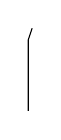
\begin{tikzpicture}[x=1cm,y=1cm]\draw (0.05,0)--(0,-0.15)--(0,-1.05);\end{tikzpicture}}}}

The sufficiency has already been stated with Kostant's theorem. For necessity, let $h'\handwritten{\leq}h$ be the order of the eigenvalue, then $c^{h'}$ centralizes $x$, hence, $x$ being regular, we have $c^{h'}=1$, hence $h'=h$, which was to be proved.

\uline{Corollary}. \deleted{\unsure{Let us consider}} \deleted{Let $D$ be a}\inserted{Let $D$ be a} regular line in $V\otimes\underline{C}$ such that there exists an ele%
% archive sheet number: 1
